\chapter{Nonlinear dynamical systems on the plane}
For this chapter the general setup will be 
\begin{align}
	\dot{x} = f(x);\quad x \in \mathbb{R}^{2};\quad f\in \mathcal{C}^1.
\end{align}
\section{One degree of freedom conservative mechanical systems}
Write $x = 
\begin{pmatrix}
	x_1 \\ x_2
\end{pmatrix}
$, with $x_1$ denoting the position and $x_2=\dot{x}_1$ denoting the speed. The total mechanical energy is given by $E(x) = \frac{1}{2}mx_2^2  + V(x_1)$, with the mass $m$ and the potential function $V$. Newton's law then gives the equations of motion 
\begin{align}
	m \ddot{x}_1 = -\frac{dV(x_1)}{dx_1} \implies 
	\begin{dcases}
		\dot{x}_1 = x_2 \\
		\dot{x}_2 = - \frac{1}{m} \frac{dV(x_1)}{dx_1}.
	\end{dcases}
\end{align}
All of the forces derive from a time-independent potential. The energy is a first integral (conserved quantity of such systems), i.e.
\begin{align}
	\frac{d}{dt}E(x(t)) = \frac{\partial E}{\partial x_1}\dot{x}_1 + \frac{\partial E}{\partial x_2}\dot{x}_2 = 0.
\end{align}
Therefore on any given trajectory $x(t)$ the energy $E(x(t))=E_0 $ is constant. Hence we can derive an explicit equation for the velocity along a trajectory which suppresses the time dependence
\begin{align}
	x_2 = \pm \sqrt{\frac{2}{m}(E_0 -V(x_1))}.
\end{align}
This leads to multiple consequences for these systems
\begin{enumerate}
	\item Trajectories form symmetric pairs (w.r.t. the $x_1$-axis) of the same energy.
	\item There is a clockwise orientation for trajectories due to 
		\begin{align}
			\dot{x}_1 = x_2 \implies
			\begin{cases}
				x_2>0 \implies x_1  \textrm{ increases} \\
				x_2 <0 \implies x_1  \textrm{ decreases} .
			\end{cases}
		\end{align}
		This is shown graphically in Fig. \ref{fig:mech_clock_orient}.
		\begin{figure}[h!]
			\centering
			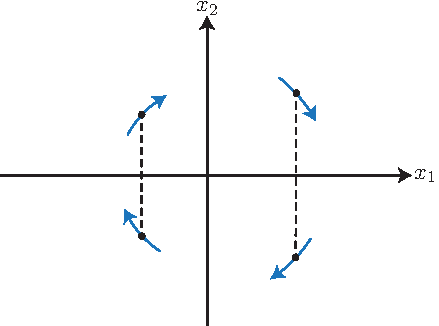
\includegraphics[width=0.6\textwidth]{figures/ch4/1mech_clock_orient.pdf}
			\caption{The clockwise orientation of trajectories in 1 degree of freedom conservative mechanical systems.}
			\label{fig:mech_clock_orient}
		\end{figure}
	\item Local minima of the potential give rise to a center fixed point surrounded by closed orbits. The minimum $x^{*} $ is a fixed point if $x^{*}_2 = 0$ (which occurs if $V(x^*_1) = E_0$) as $\dot{x}_2 \propto V'(x^{*}_1) = 0 $. The trajectories of the closed orbits can be found using $x_2 = \pm \sqrt{\frac{2}{m}(E_0 - V(x_1))}$. Such a fixed point at a local minimum of the potential surrounded by closed orbits is shown in Fig. \ref{fig:mech_loc_extrem}.
\begin{figure}[h!]
	\centering
	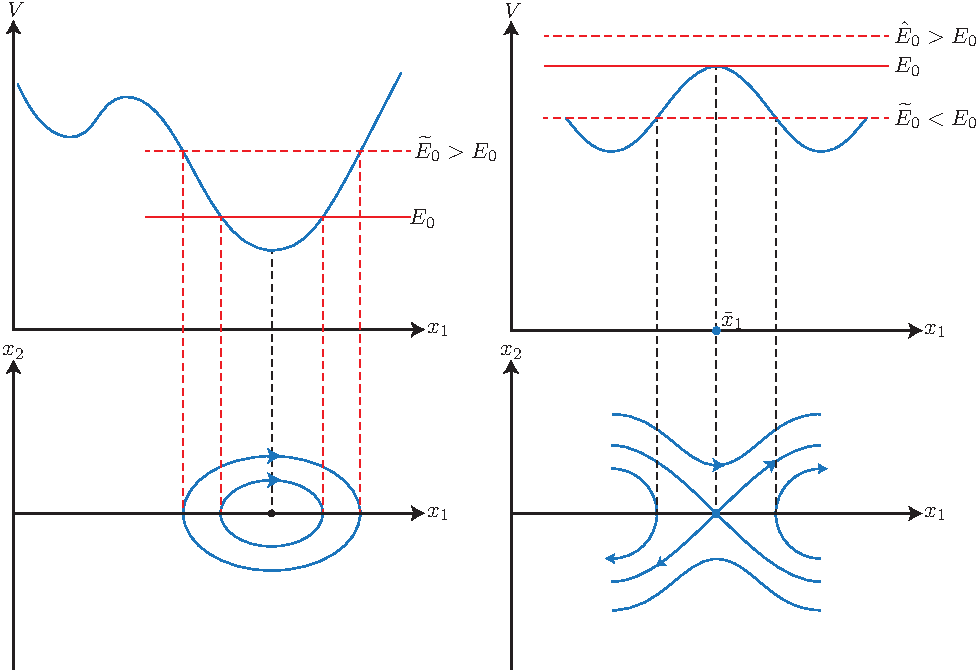
\includegraphics[width=0.99\textwidth]{figures/ch4/3mech_orbits.pdf}
	%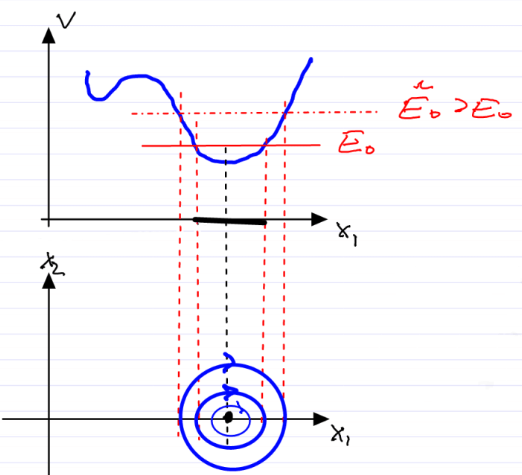
\includegraphics[width=0.47\textwidth]{figures/ch4/2mech_orbits_minima.png}
	%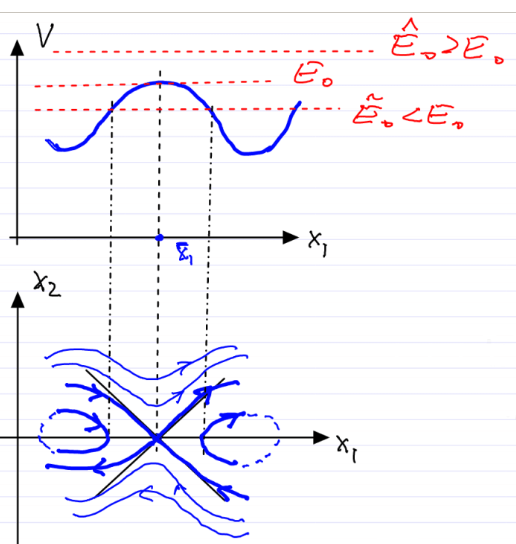
\includegraphics[width=0.39\textwidth]{figures/ch4/3mech_orbits_maxima.png}
	\caption{Left: Closed orbits around the fixed point at the local minimum of the potential function. Right: The saddle type fixed point at the local maxima of the potential. The clockwise orientations comes from consequence (ii).}
	\label{fig:mech_loc_extrem}
\end{figure}
\item At local maxima of the potential saddle type fixed points arise. The maximum $x^{*}$ is a fixed point if $x^{*}_2=0 $ (which occurs if $V(x^*_1)=E_0$) as $V'(x^{*}_2)=0$. The velocity can be approximated as follows
	\begin{subequations}
	 \begin{align}
		 x_2 &= \pm \sqrt{\frac{2}{m}(E_0 -V(x_1))} \\
		     &= \pm \sqrt{\frac{2}{m}} \sqrt{\underbrace{(E_0 - V(x^{*}_1))}_{=0} - \underbrace{V'(x^{*}_{1})}_{=0}(x_1 - x^{*}_1) - \frac{1}{2}\underbrace{V''(x^{*}_1)}_{<0}(x_1 - x^{*}_{1})^2 + \mathcal{O}((x_1 - x^{*}_1)^3)} \\
		     &=\pm \sqrt{\frac{2}{m}}\sqrt{-\frac{V''(x^{*}_1)}{2}}\left|x_1 - x^{*}_1\right| +  \textrm{higher order terms} .
	\end{align}
\end{subequations}
The behavior is sketched in Fig. \ref{fig:mech_loc_extrem}
\item A local minimum has local maxima to the left and right, unless $V$ is monotonously nondecreasing to infinity. Then we have two cases to differentiate. One where the local maxima are at the same level, and the other where one local maximum has a smaller potential than the other (or in one direction $V$ monotonously increases towards infinity). \emph{Homoclinic orbits} are special periodic orbits that are formed on a level set that contains a single saddle point. \emph{Heteroclinic orbits} are formed when the level set contains two saddle points, i.e. when the two maxima have the same potential. These two cases are illustrated in Fig. \ref{fig:mech_limit_case}. 
	\begin{figure}[h!]
		\centering
		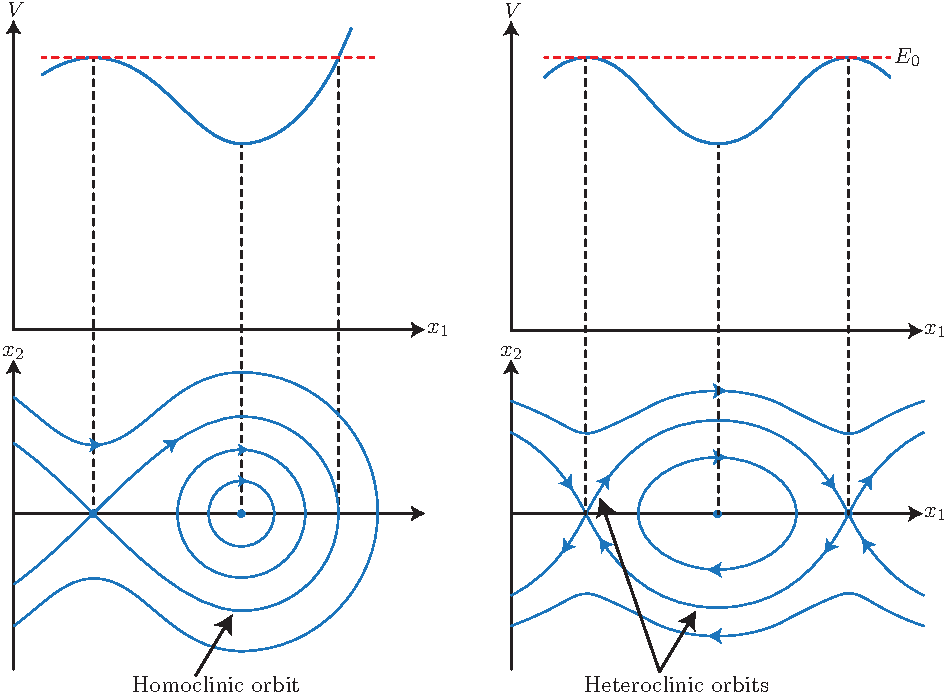
\includegraphics[width=0.99\textwidth]{figures/ch4/4mech_limit_case.pdf}
		\caption{Left: One maximum has a lower potential than the other (or $V$ is nondecreasing towards infinity on the right). The black arrow denotes a homoclinic orbit. Right: All maxima have the same potential. The black arrows denote heteroclinic orbits.}
		\label{fig:mech_limit_case}
	\end{figure}
	
\end{enumerate}

These consequences are illuminated in a basic example.
\begin{ex}[The Duffing oscillator]
Let the equation of motion be given by
\begin{align}
\ddot{x}-x+x^3=0;\quad x_1=x;\quad x_2=\dot{x}.	
\end{align}
Therefore we get the first order ODE
\begin{align}
	\begin{dcases}
		\dot{x}_1 = x_2 \\
		\dot{x}_2 = x_1 - x_1^3 = - V'(x_1)
	\end{dcases}
	\implies E(x) = \frac{1}{2}x_2^2+ V(x_1) = \frac{1}{2}x_2^2 + \left( - \frac{1}{2}x_1^2 + \frac{1}{4}x_1^4\right).	
\end{align}
The full phase portrait with two homoclinic orbits is shown in Fig. \ref{fig:duffing_phase_portrait}. 
We find two stable fixed points at the potential minima and they are separated by a potential maximum in the middle. Periodic orbits surround the stable fixed points. These orbits are separated from the rest of the phase space by the two homoclinic orbits of the saddle. Outside, we have periodic orbits that correspond to energy level-sets higher than the potential of the saddle. 
\begin{figure}[h!]
	\centering
	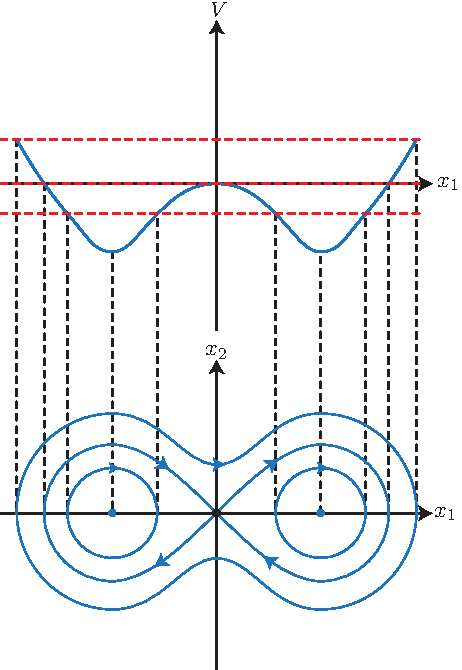
\includegraphics[width=0.6\textwidth]{figures/ch4/5duffing_phase_portrait.pdf}
	\caption{Phase portrait of the Duffing oscillator using the potential $V$.}
	\label{fig:duffing_phase_portrait}
\end{figure}

\end{ex}

\section{Global behavior in two dimensional autonomous dynamical systems}
Consider the following dynamical system
\begin{align}
	\dot{x} = f(x);\quad x \in \mathbb{R}^{2};\quad f \in \mathcal{C}^1.
\end{align}
Further assume that solutions exist for all times, therefore there exists a unique solution $x(t; x_0)$ for all $t \in \mathbb{R}$ such that $x(0;x_0)=x_0$. Next, a few definitions are introduced enabling a deeper exploration of such systems.

\begin{definition}
	A point $p \in \mathbb{R}^{2}$ is an \emph{$\omega$-limit point} of $x_0$ if there exists a monotone increasing unbounded sequence of times $\{t_i\}_{i=1}^{\infty}$ with $t_1 \geq 0$ such that 
	\begin{align}
		\lim_{i\to \infty}x(t_i;x_0)=p.
	\end{align}
\end{definition}

\begin{definition}
	A point $q \in \mathbb{R}^{2}$ is an \emph{$\alpha$-limit point} of $x_0$ if it is an $\omega $-limit point in backward time. 
\end{definition}

\begin{definition}
	The \emph{$\omega $-limit set} of $x_0$, denoted $\omega(x_0)$ is the set of all $\omega$-limit points of $x_0$.
	The \emph{$\alpha $-limit set} of $x_0$, denoted $\alpha(x_0)$ is the set of all $\alpha$-limit points of $x_0$.
\end{definition}
\begin{remark}[]
	Note that $\omega(x_0)$ and $\alpha(x_0)$ is the same for all $x_0 $ along a given trajectory, thus limit sets can be associated with full trajectories.
\end{remark}
\begin{ex}[Examples of limit sets]
	Below (Fig. \ref{fig:limset_ex}) three different limit sets are depicted.
	\begin{figure}[h!]
		\centering
		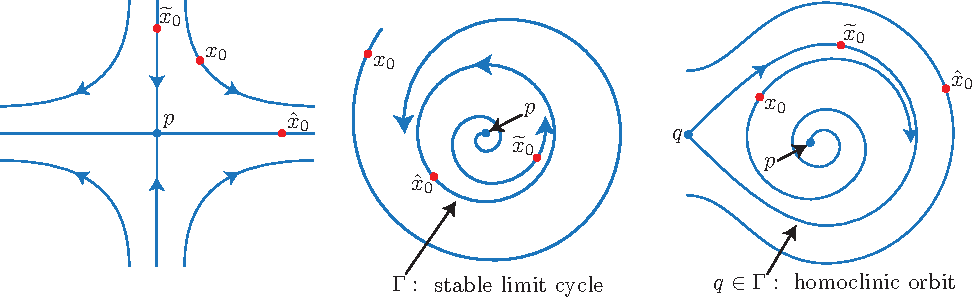
\includegraphics[width=0.99\textwidth]{figures/ch4/6limset_ex.pdf}
		%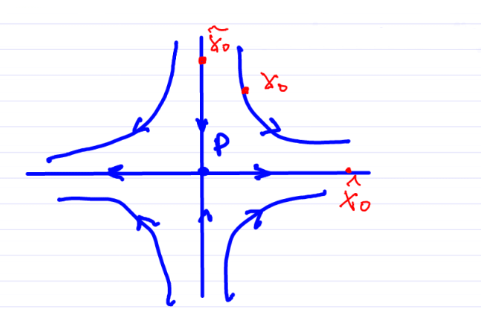
\includegraphics[width=0.3\textwidth]{figures/ch4/6limset_ex_1.png}
		%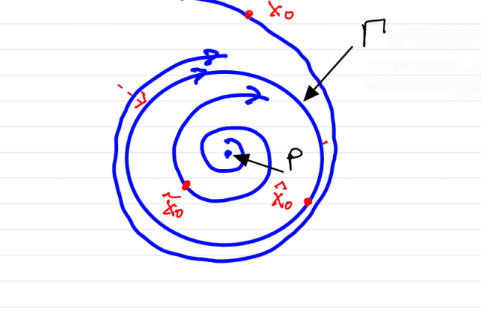
\includegraphics[width=0.3\textwidth]{figures/ch4/6limset_ex_2.png}
		%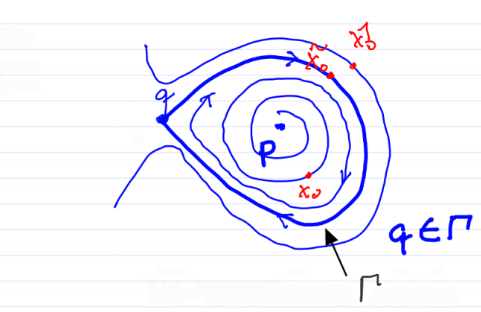
\includegraphics[width=0.3\textwidth]{figures/ch4/6limset_ex_3.png}
		\caption{Three example systems for which we examine the respective limit sets. The arrows labelled $\Gamma $ denote a stable limit cycle (middle) and a homoclinic orbit (right).}
		\label{fig:limset_ex}
	\end{figure}
	For the leftmost dynamical system we have $\omega(p)=\alpha(p)=\{p\}$ and
	\begin{subequations}
\begin{align}
	\omega(x_0) &= \emptyset, \quad &\omega(\tilde{x}_0) &= \{p\}, \quad &{\omega }(\hat{x}_0)&= \emptyset, \\
	\alpha(x_0)&=\emptyset, \quad & \alpha(\tilde{x}_0)&=\emptyset,\quad &\alpha(\hat{x}_0&=\{p\}.
\end{align}
\end{subequations}
	For the middle dynamical system we have 
	\begin{subequations}
\begin{align}
	\omega(x_0) &= \Gamma, \quad &\omega(\tilde{x}_0) &= \Gamma, \quad &{\omega }(\hat{x}_0)&= \Gamma, \\
	\alpha(x_0)&= \textrm{unclear} , \quad & \alpha(\tilde{x}_0)&=\{p\},\quad &\alpha(\hat{x}_0)&=\Gamma.
\end{align}
\end{subequations}
	For the rightmost dynamical system we have 
	\begin{subequations}
\begin{align}
	\omega(x_0) &= \Gamma, \quad &\omega(\tilde{x}_0) &= \{q\}, \quad &{\omega }(\hat{x}_0)&=  \textrm{unclear}, \\
	\alpha(x_0)&= \{p\} , \quad & \alpha(\tilde{x}_0)&=\{q\},\quad &\alpha(\hat{x}_0)&= \textrm{unclear} .
\end{align}
\end{subequations}
\end{ex}

We now introduce two theorems which give us more insight into these limit sets.
\begin{theorem}[]
	If $x(t;x_0)$ is bounded, then $\omega(x_0)$ and $\alpha(x_0)$ are nonempty, closed, and connected. Further, the omega and alpha limit sets are invariant sets, i.e. they consist of full trajectories.
\end{theorem}
\begin{theorem}[Poincaré-Bendixon]
	If $x(t;x_0)$ is bounded, then $\omega(x_0)$ and $\alpha(x_0)$ must be one of the following 
	\begin{enumerate}
		\item A connected set of fixed points,
		\item A limit cycle,
		\item A set of fixed points and their homo-/heteroclinic orbits (illustrated in Fig. \ref{fig:poincare-bendixon}).
	\end{enumerate}
	There is no complex (chaotic) liminting behavior in 2-dimensional autonomous nonlinear systems. 
	\begin{figure}[h!]
		\centering
		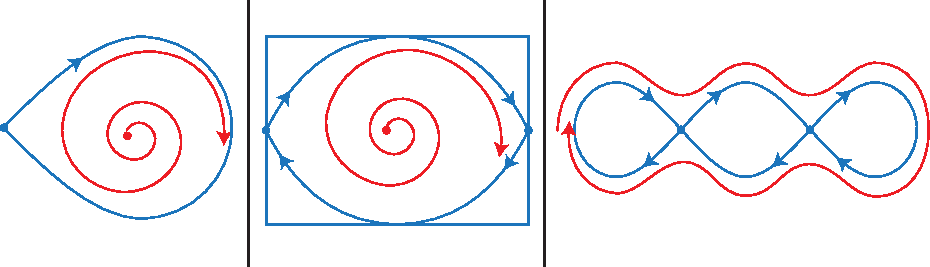
\includegraphics[width=0.99\textwidth]{figures/ch4/8poincare-bendixon.pdf}
		\caption{Examples of a set of fixed points connected by homo-/heteroclinic orbits.}
		\label{fig:poincare-bendixon}
	\end{figure}	
\end{theorem}
\begin{remark}[]
	The homo-/heteroclinic orbits are generally not robust, thus we should not expect to see them in a typical dynamical system. We can imagine that under small perturbations the continuous line of the orbit breaks up into separate unstable and stable manifolds as shown in Fig. \ref{fig:pd_robust}.
	\begin{figure}[h!]
		\centering
		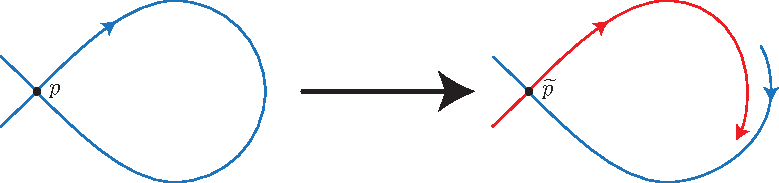
\includegraphics[width=0.99\textwidth]{figures/ch4/9pd_robust.pdf}
		\caption{The loss of the homoclinic orbit under a small perturbation. Before the perturbation $\Gamma=W^{S}(p)=W^{U}(p)$ ($p$ is the hyperbolic fixed point), meanwhile after the perturbation $W ^{S}(p) \neq W^{U} (p)$. The unstable manifold is given in red, and the stable manifold in blue.}
		\label{fig:pd_robust}
	\end{figure}
	However, these orbits are robust within the class of conservative systems, and conservative pertubations do not lead to global bifurcations as seen in Fig. \ref{fig:pd_conservative}.
	\begin{figure}[h!]
		\centering
		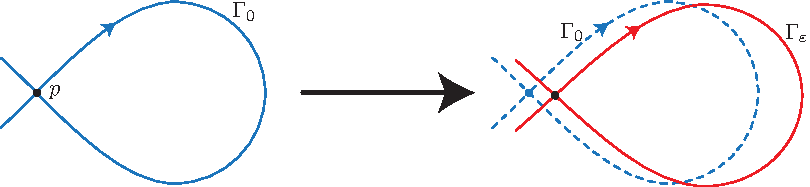
\includegraphics[width=0.99\textwidth]{figures/ch4/10pd_conservative.pdf}
		\caption{Small conservative perturbation does not lead to a global bifurcation in conservative systems. The energy level containing $\Gamma_0$ is robust, and perturbs to a new $\Gamma_\varepsilon$.}
		\label{fig:pd_conservative}
	\end{figure}
	
\end{remark}
\begin{remark}[]
	A consequence of the Poincaré-Bendixon Theorem is that a forward-invariant, bounded open set without fixed points \underline{must} contain a limit cycle. This is due to the elimination of possibilities (i) and (iii) in the theorem. An example of such a set is shown in Fig. \ref{fig:PB_consequence}.
	\begin{figure}[h!]
		\centering
		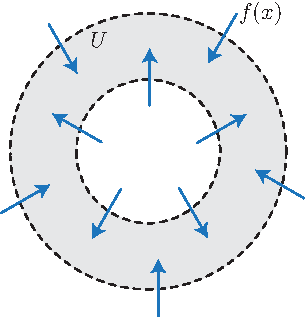
\includegraphics[width=0.6\textwidth]{figures/ch4/11PB_consequence.pdf}
		\caption{A forward-invariant, bounded open set without fixed points as in the remark. Such a set must contain a limit cycle.}
		\label{fig:PB_consequence}
	\end{figure}
	
\end{remark}
\begin{proposition}[Bendixson criterion]
	Consider the following
	\begin{align}
		\dot{x}	= f(x);\quad x\in \mathbb{R}^{2}; f\in \mathcal{C}^{1};\quad U  \textrm{ simply connected} .
	\end{align}
And further assume 
% everywhere with nabla cdot use  \textrm{div } 
 \begin{align}
	  x\in U \implies  \nabla \cdot  f(x) \neq 0.
\end{align}
This in turn implies $\nabla \cdot f(x)$ has constant sign on $U$. Then there cannot exist a limit cycle in $U$.
\end{proposition}
\begin{proof}
	Assume, towards a contradiction, that there exists a closed orbit $\Gamma$ of period $\tau$. Calculate 
	\begin{align}
	f^{\perp}(x) =
	\begin{pmatrix}
		f_2(x) \\ -f_1(x)
	\end{pmatrix}
	\implies \oint_{\Gamma }f^{\perp}\cdot \underbrace{dr}_{=\dot{r}dt}
	=\int_{0}^{\tau} f^{\perp}(r(t)) \cdot f(r(t)) dt = 0.
	\end{align}
On the other hand we have by Green's Theorem
\begin{align}
	\oint_{\Gamma }f^{\perp}\cdot dr = \int \int_{\Gamma^{\degree}} \left(\nabla \times f^{\perp}\right)_{z}dA = - \int \int_{\Gamma^{\degree}} \underbrace{\nabla \cdot f}_{\neq 0}dA \neq 0.
\end{align}
Here, $\Gamma^{\degree}$ denotes the interior of the area enclosed by $\Gamma$. These two equations stand in contradiction to each other, therefore no limit cycle can exist in $U$. 
\end{proof}
\begin{remark}[]
	Another consequence of the Poincaré-Bendixson Theorem is that purely damped or purely forced perturbations of a conservative system cannot have limit cycles. 
	\begin{align}
		f(x) =
		\begin{dcases}
			\dot{x}_1 = x_2 \\
			\dot{x}_2 = -V'(x_1) + g(x_1, x_2)
		\end{dcases}
		;\quad 
		\nabla \cdot f = \nabla \cdot
		\begin{pmatrix}
			0 \\ g(x)
		\end{pmatrix}
		=\frac{\partial g}{\partial x_2}.
	\end{align}
	If we assume pure damping or forcing, the divergence of $f$ cannot be 0 on any open set. If it is positive, we have pure forcing, alternatively if it is negative we have pure damping. In either case no limit cycle can exist.	
\end{remark}

